\documentclass[aspectratio=169]{beamer}
\usepackage{fontspec}
\setmainfont{Yanone Kaffeesatz}
\setsansfont{Noto Sans}
\setmonofont{Fira Code}
%%% Fonts and language setup.
\usepackage{polyglossia}
%% Math
\usepackage{amsmath, amsfonts, amssymb, amsthm, mathtools} % Advanced math tools.
\usepackage{unicode-math} % Allow TTF and OTF fonts in math and allow direct typing unicode math characters.
\unimathsetup{
    warnings-off={
            mathtools-colon,
            mathtools-overbracket
        }
}
\setmathfont{Fira Math}
\newfontfamily{\cyrillicfont}{Fira Math}


\usetheme{Rochester}
\usecolortheme[style=light]{Nord}
\usefonttheme{Nord}
\setbeamertemplate{navigation symbols}{}%remove navigation symbols


\usepackage{minted}
\usemintedstyle{nord}

\title{Roslyn}
\author{Николай Пономарев}
\date{}


%%% Polyglossia setup after (nearly) everything as described in documentation.
\setdefaultlanguage{russian}
\setotherlanguage{english}

\begin{document}

\maketitle

\begin{frame}{Roslyn}
        .NET Compiler Platform (или Roslyn)~--- open--source реализация компиляторов C\# и Visual Basic, которая предоставляет богатый API для кодогенерации и анализа кода.
\end{frame}

\begin{frame}{Возможности}
    Roslyn SDK позволяет создавать
    \begin{itemize}
        \item анализаторы
        \item исправления кода
        \item рефакторинг кода
    \end{itemize}
    на основе статического анализа кода
    Так же есть инструменты для генерации кода
\end{frame}

\begin{frame}{Модель API компилятора}
    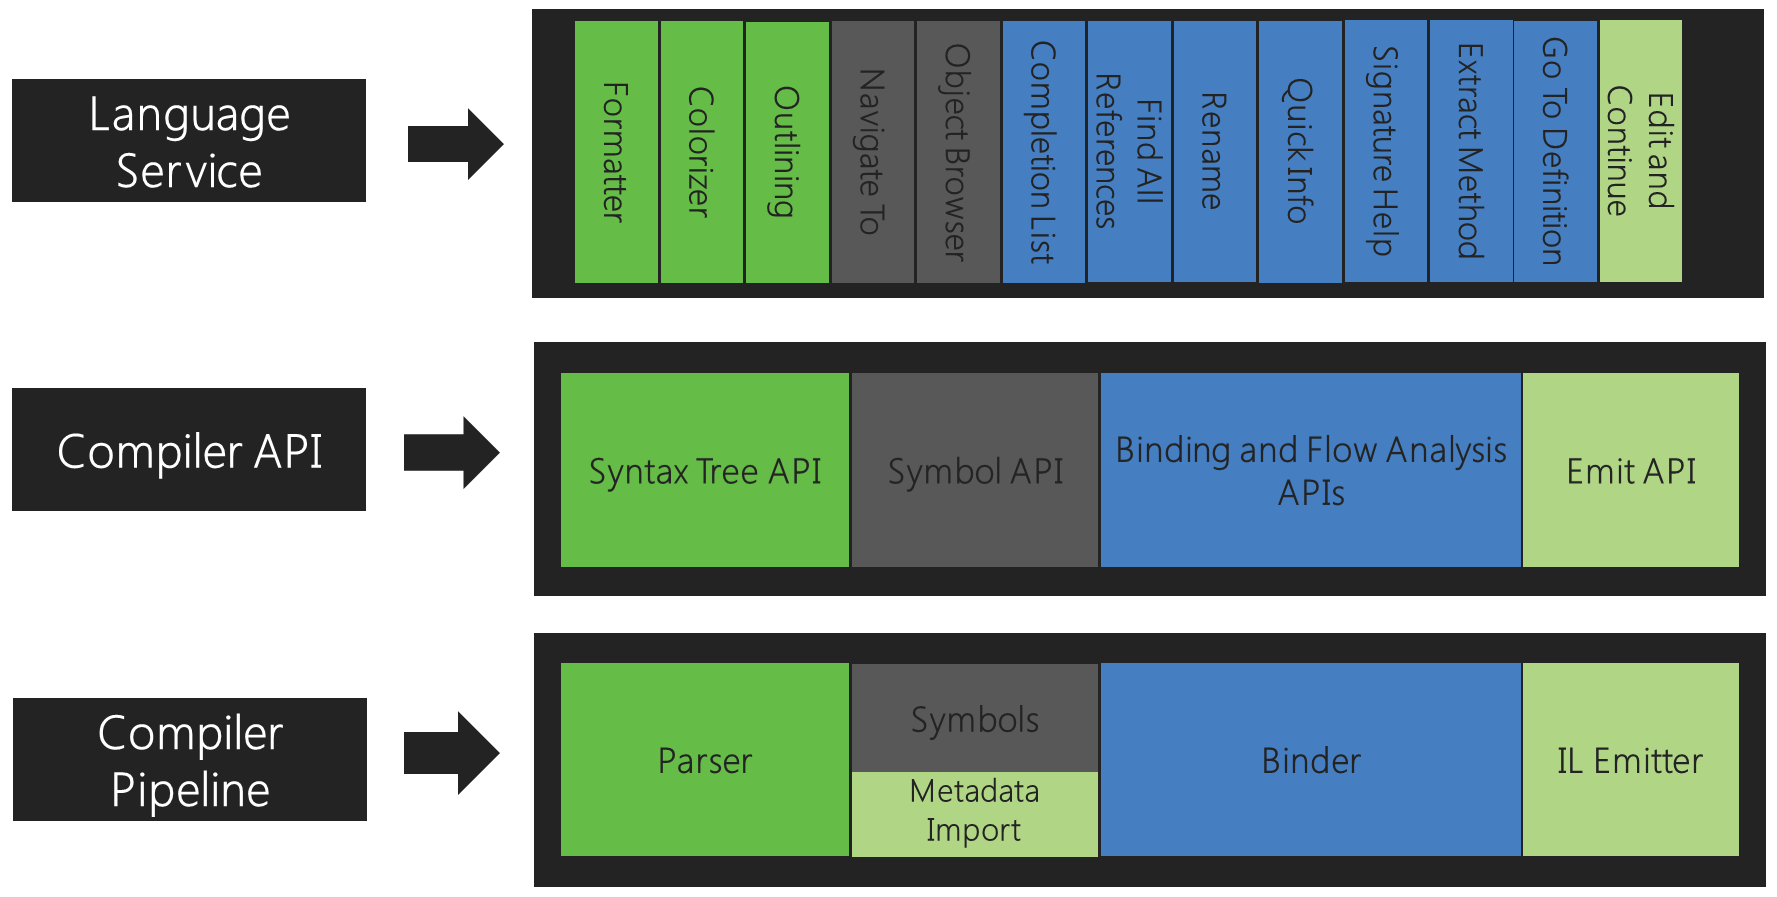
\includegraphics[width=\textwidth]{compiler-pipeline-lang-svc.png}
\end{frame}

\begin{frame}{APIs}
    \begin{itemize}
        \item Syntax API
            \begin{itemize}
                \item отвечает за представление кода в качестве синтаксического дерева, содержащего полный исходный код программы
            \end{itemize}
        \item Symbol API
            \begin{itemize}
                \item позволяет исследовать свойства объекта
            \end{itemize}
        \item Binding \& Flow Analysis APIs
            \begin{itemize}
                \item позволяют исследовать, что происходит с объектом в процессе исполнения программы
            \end{itemize}
        \item Emit API
            \begin{itemize}
                \item позволяет <<производить>> сборки из синтаксических деревьев
            \end{itemize}
    \end{itemize}
\end{frame}

\begin{frame}{Использование}
    \begin{itemize}
        \item Статический анализ для IDE 
        \item Анализаторы 
            \begin{itemize}
                \item Соблюдение стандартов кода в проекте
                \item Подсказки при использовании сторонних библиотек
                \item Best practices
            \end{itemize}
        \item Прикладные задачи
            \begin{itemize}
                \item Рефакторинг старого кода
                \item Миграции на новые версии библиотек/языка
            \end{itemize}
    \end{itemize}
\end{frame}

\begin{frame}{Полезные ссылки}
    \begin{itemize}
        \item \href{https://learn.microsoft.com/en-us/dotnet/csharp/roslyn-sdk/}{Документация в MSDN}
        \item \href{https://joshvarty.com/learn-roslyn-now/}{Цикл статей Learn Roslyn Now}
        \item \href{https://github.com/ironcev/awesome-roslyn}{Список ресурсов Awesome Roslyn}
        \item \href{https://habr.com/ru/company/veeam/blog/648775/}{Статья на Хабре про <<быстрый>> рефакторинг с использованием кодогенераторов}
        \item \href{https://lizzy-gallagher.github.io/roslyn-refactoring/}{Еще одна статья про рефакторинг}
    \end{itemize}
\end{frame}

\end{document}
